\taskpic{Сверхпроводящее кольцо радиуса $l$ помещено в однородное
  горизонтальное магнитное поле с индукцией $B$. Ось кольца
  параллельна линиям магнитной индукции поля. Стержень массой $m$ и
  длиной $l$, имеющий сопротивление $R$, закреплен одним концом в
  центре кольца и может без трения поворачиваться вокруг этой точки,
  сохраняя электрический контакт с кольцом. По какому закону должно
  изменяться напряжение $U$, приложенное между кольцом и его центром,
  чтобы стержень вращался с постоянной угловой скоростью $\omega$?
  Ускорение свободного падения равно $g$.}{
  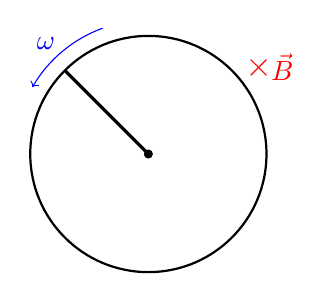
\begin{tikzpicture}
    \draw[thick] (0,0) circle (1.5);
    \draw[very thick] (0,0) -- ({1.5*cos(135)},{1.5*sin(135)});
    \draw[blue,->] ({1.7*cos(110)},{1.7*sin(110)}) arc (110:150:1.7);
    \draw[blue] (-1.3,1.4) node {$\omega$};
    \draw[red] (1.3,1) -- ++(0.2,0.2);
    \draw[red] (1.3,1.2) -- ++(0.2,-0.2);
    \draw[red] (1.7,1.1) node {$\vec{B}$};
    \draw[fill=black] (0,0) circle (0.05);
  \end{tikzpicture}
}